\section{Comportamento caotico del sistema}

Si suppone che la resistenza $R$ del sistema vari periodicamente del 25\% seguendo la legge:
\begin{equation}
    R(t) = \bar{R} (1+0.25 \sin(\omega t))
    \label{eq:resistenza-var}
\end{equation}

Per mantenere il sistema autonomo e poterlo quindi simulare, si possono introdurre due nuove equazioni relative a due nuove variabili di stato, disaccoppiate dalle precedenti.
Il sistema diventa dunque:

\begin{equation}
    \left\{
    \begin{aligned}
        R =& \bar{R} (1+0.25 x_4) \\
        \dot{x_1} =& -\frac{\strut R}{\strut L}x_1 + \frac{1}{L} x_2\\
        \dot{x_2} =& -\frac{\strut 1}{\strut C} x_1 + \frac{1}{C}\left( \alpha x_2 - \beta x_2^3\right)\\
        \dot{x_3} =& x_3 - \omega x_4 - (x_3^2+x_4^2) x_3 \\
        \dot{x_4} =& \omega x_3 + x_4 - (x_3^2+x_4^2) x_4 \\
    \end{aligned}
    \right.
    \label{eq:sistema-chaos}
\end{equation}

Dove è immediato verificare per sostituzione che
\begin{equation}
    \begin{aligned}
        x_3 =& \cos (\omega t)\\
        x_4 =& \sin (\omega t)\\
    \end{aligned}
\end{equation}

Dall'equazione~\ref{eq:resistenza-var} si osserva che, per valori di $\bar{R}$ ragionevoli ($29.5 \Omega$ ad esempio) l'oscillazione è sufficientemente ampia da passare per tutti i punti di biforcazione (\autoref{tab:biforc-r}): non è davvero necessario variare $\bar{R}$ per trovare il caos.

La precedente osservazione semplifica molto il problema, che si riduce a trovare attraverso delle simulazioni un giusto valore del solo parametro $\omega$ per cui il sistema presenti comportamento caotico.

I dati usati nelle simulazioni sono i seguenti:
\begin{itemize}
    \item $\alpha, \beta, L, C$ come indicati nel testo;
    \item $R=29.5 \Omega$;
    \item $\bar{x_0} = [-0.005, -0.001, 0, 1]$;
    \item $\omega \in [0.5, 5]$.
\end{itemize}

Provando a calcolare sistematicamente gli esponenti di Lyapunov del sistema~\ref{eq:sistema-chaos} per valori di $\omega$ nell'ordine di grandezza dell'unità, si ottiene il risultato illustrato in~\autoref{fig:lyapunov-plot}.

\begin{figure}
    \centering
    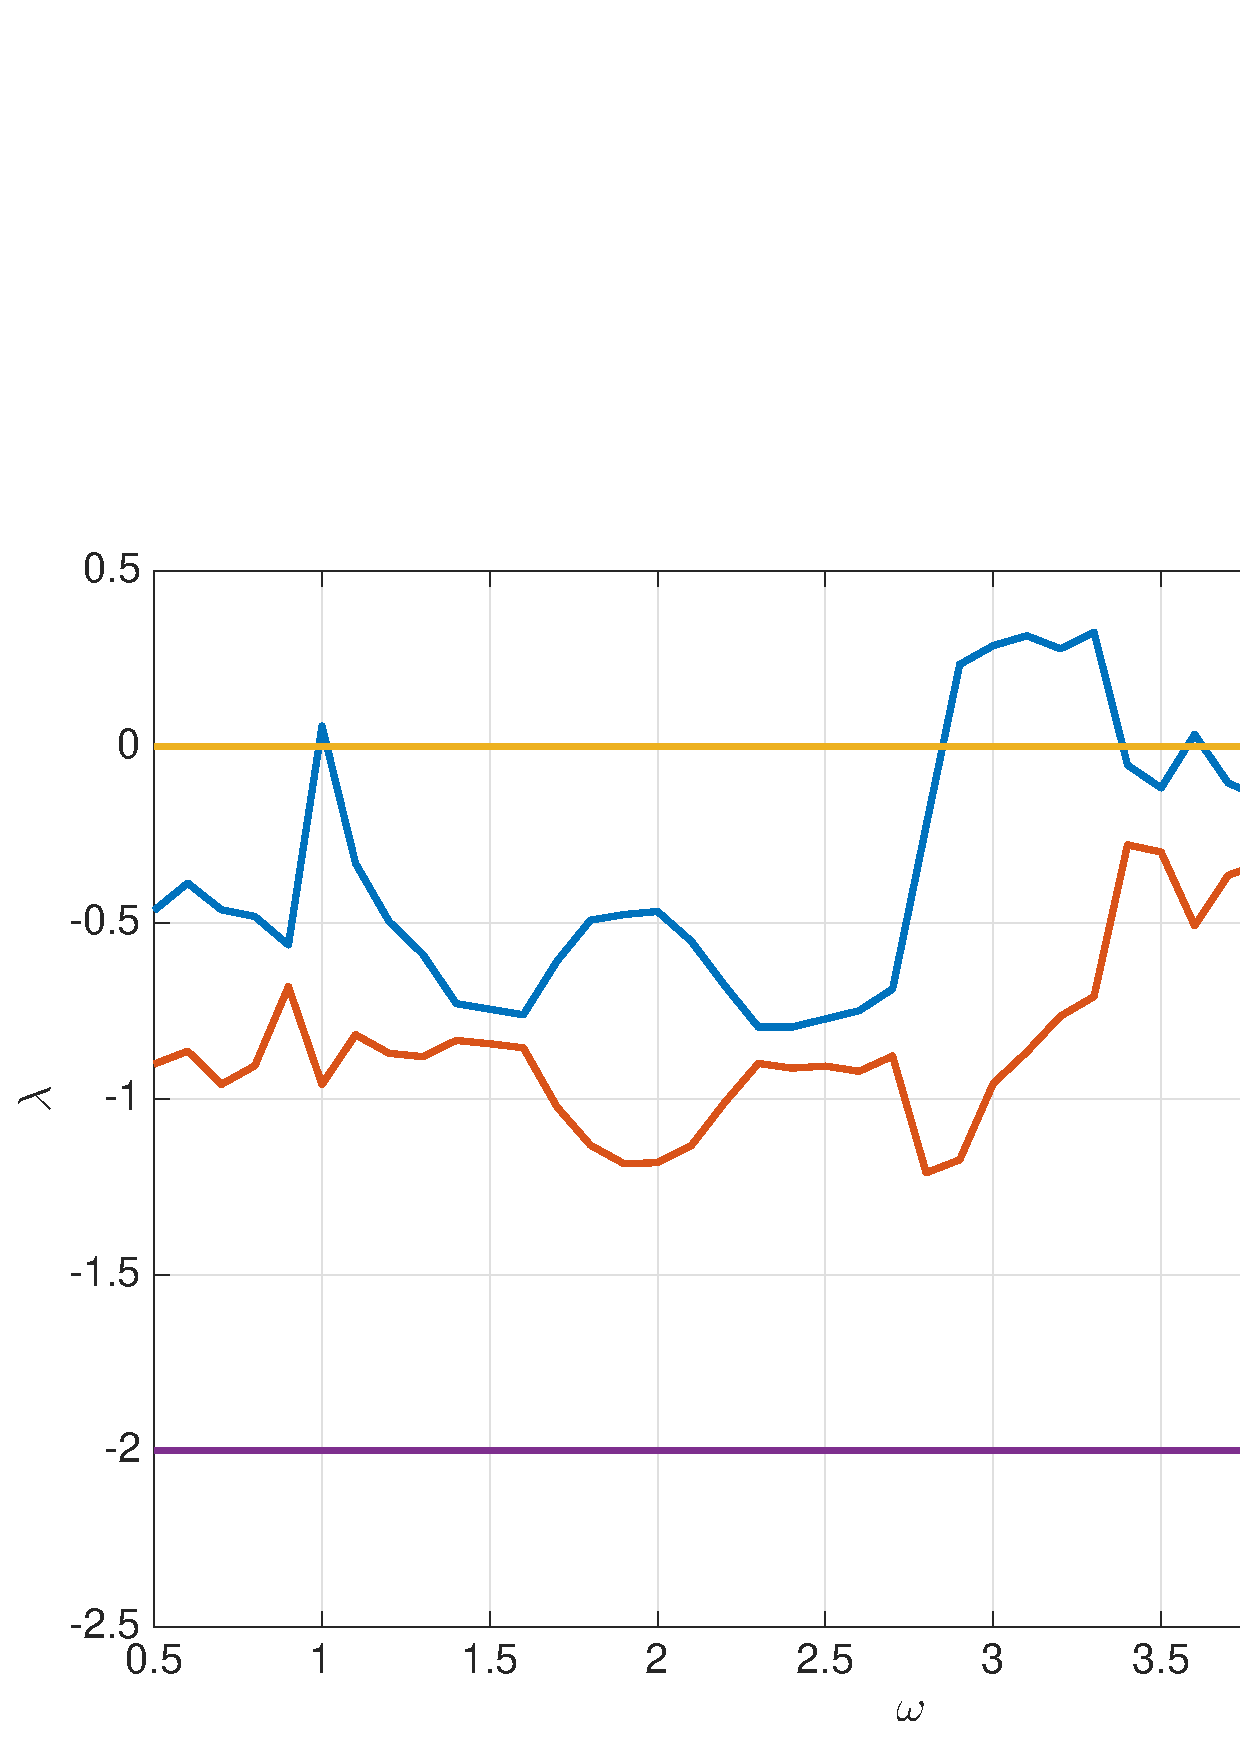
\includegraphics[width=\textwidth]{matcont/LyapunovPlot}
    \caption{Esponenti di Lyapunov del sistema~\ref{eq:sistema-chaos} calcolati per $\omega \in [0.5, 5]$, $\bar{R}=29.5 \Omega$.}
    \label{fig:lyapunov-plot}
\end{figure}

Integrando per intervalli estesi il sistema, si verifica che effettivamente per $\omega = 3.1415$ gli esponenti di Lyapunov valgono: $[0.28, 0, -0.77, -2]$.

Ciò dimostra il comportamento caotico del sistema. Lo strano attrattore simulato per gli stessi parametri è mostrato in~\autoref{fig:strano-attrattore}, insieme alla sua sezione di Poincaré in~\autoref{fig:chaos-poincare}.

\begin{figure}
    \centering
    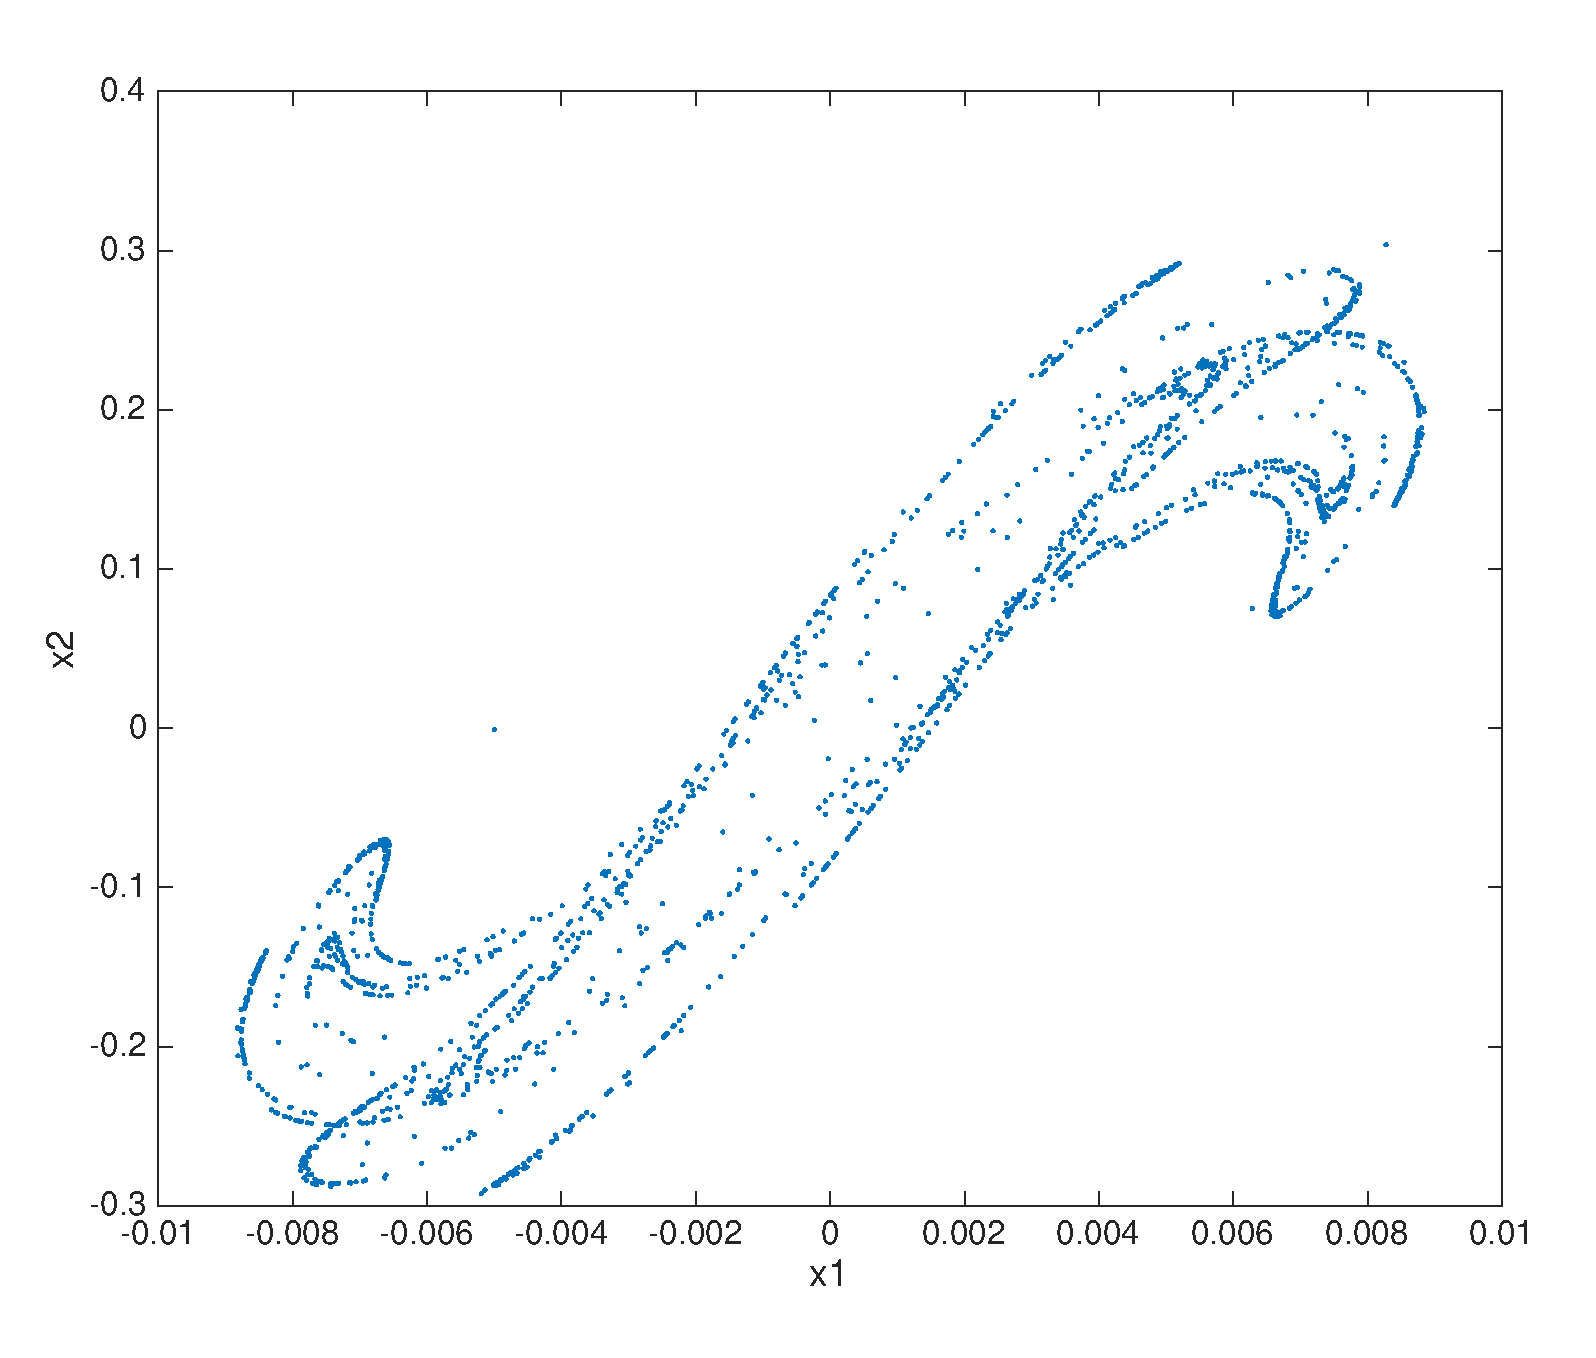
\includegraphics[width=\textwidth]{matcont/PoincareCaos}
    \caption{La mappa di Poincaré dello strano attrattore.}
    \label{fig:chaos-poincare}
\end{figure}

\begin{figure}
    \centering
    \begin{subfigure}{\textwidth}
        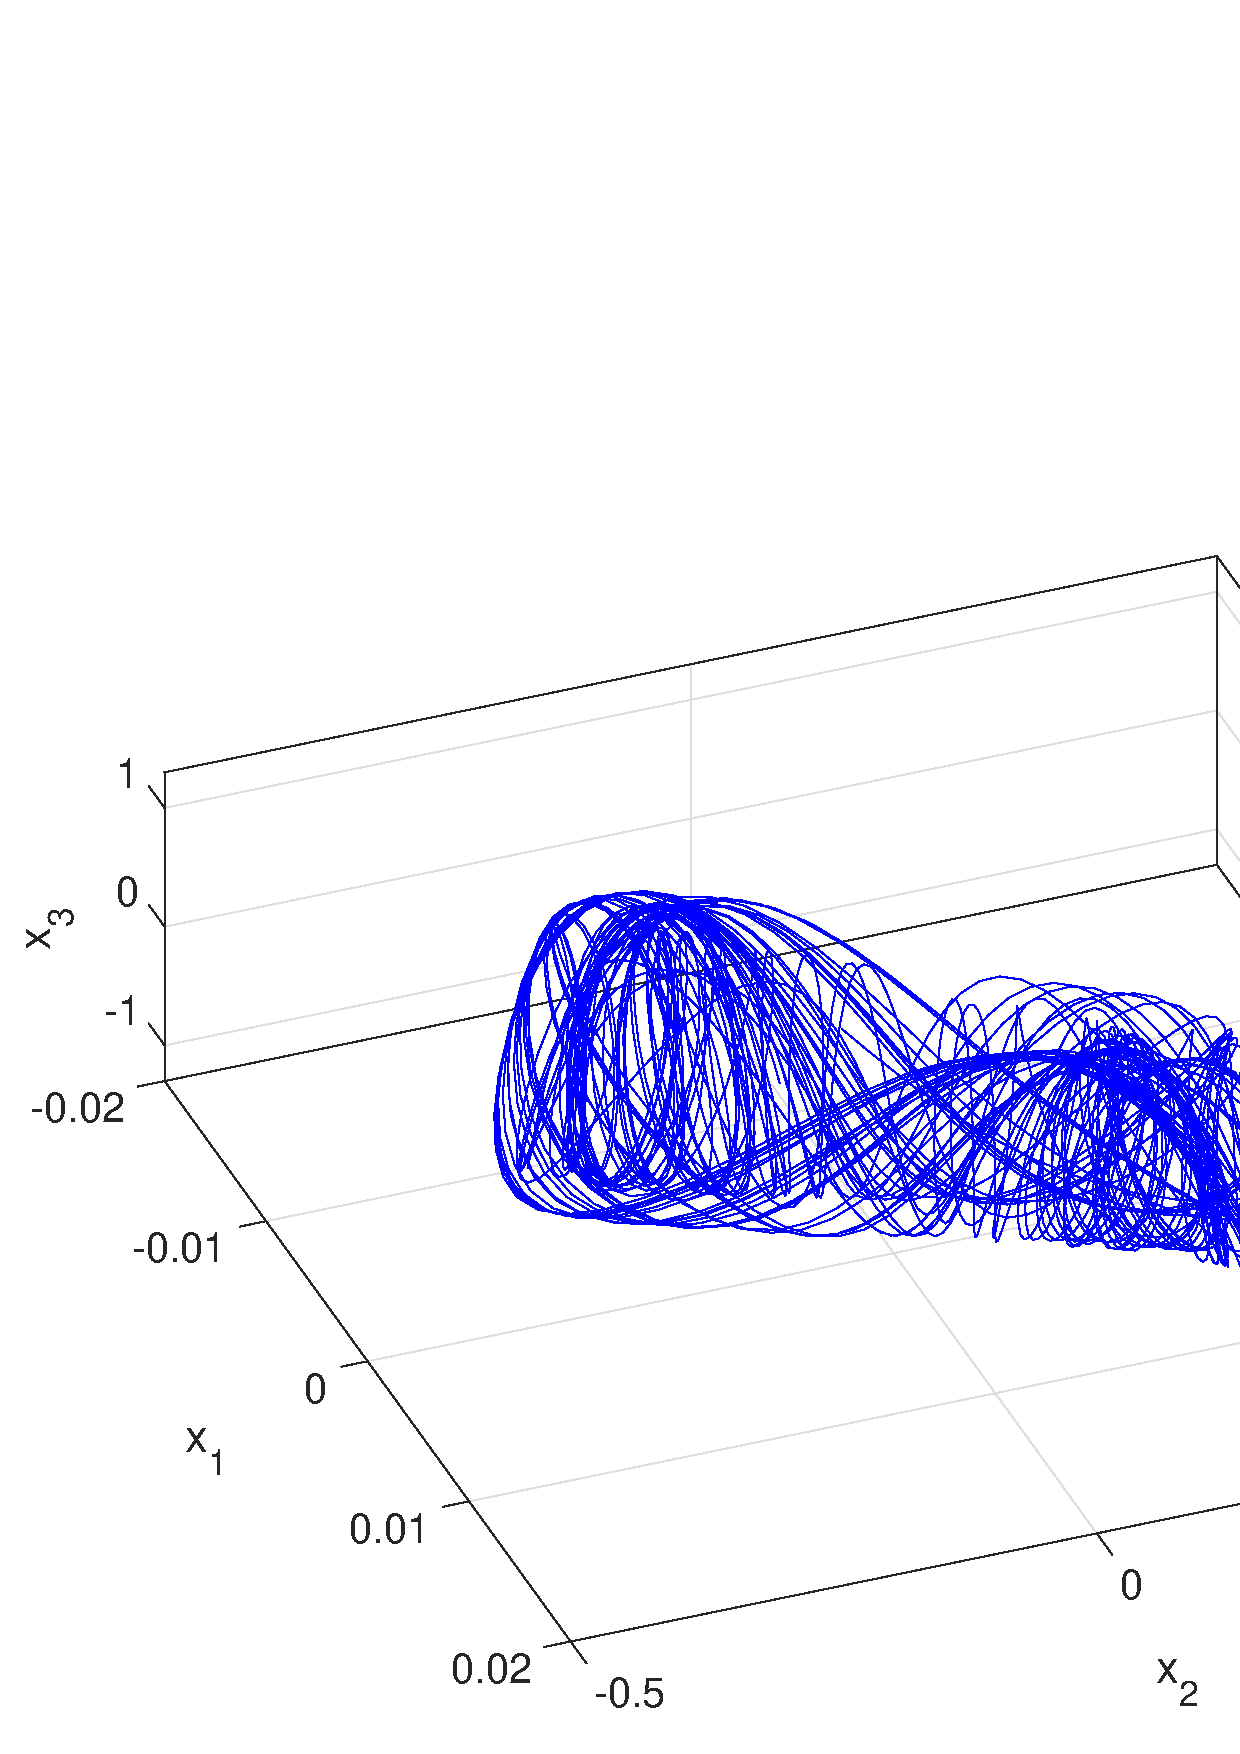
\includegraphics[width=\textwidth]{matcont/StranoAttrattore}
        \caption{Simulazione di un'orbita nello strano attrattore.}
    \end{subfigure}
    \par\bigskip
    \begin{subfigure}{0.85\textwidth}
        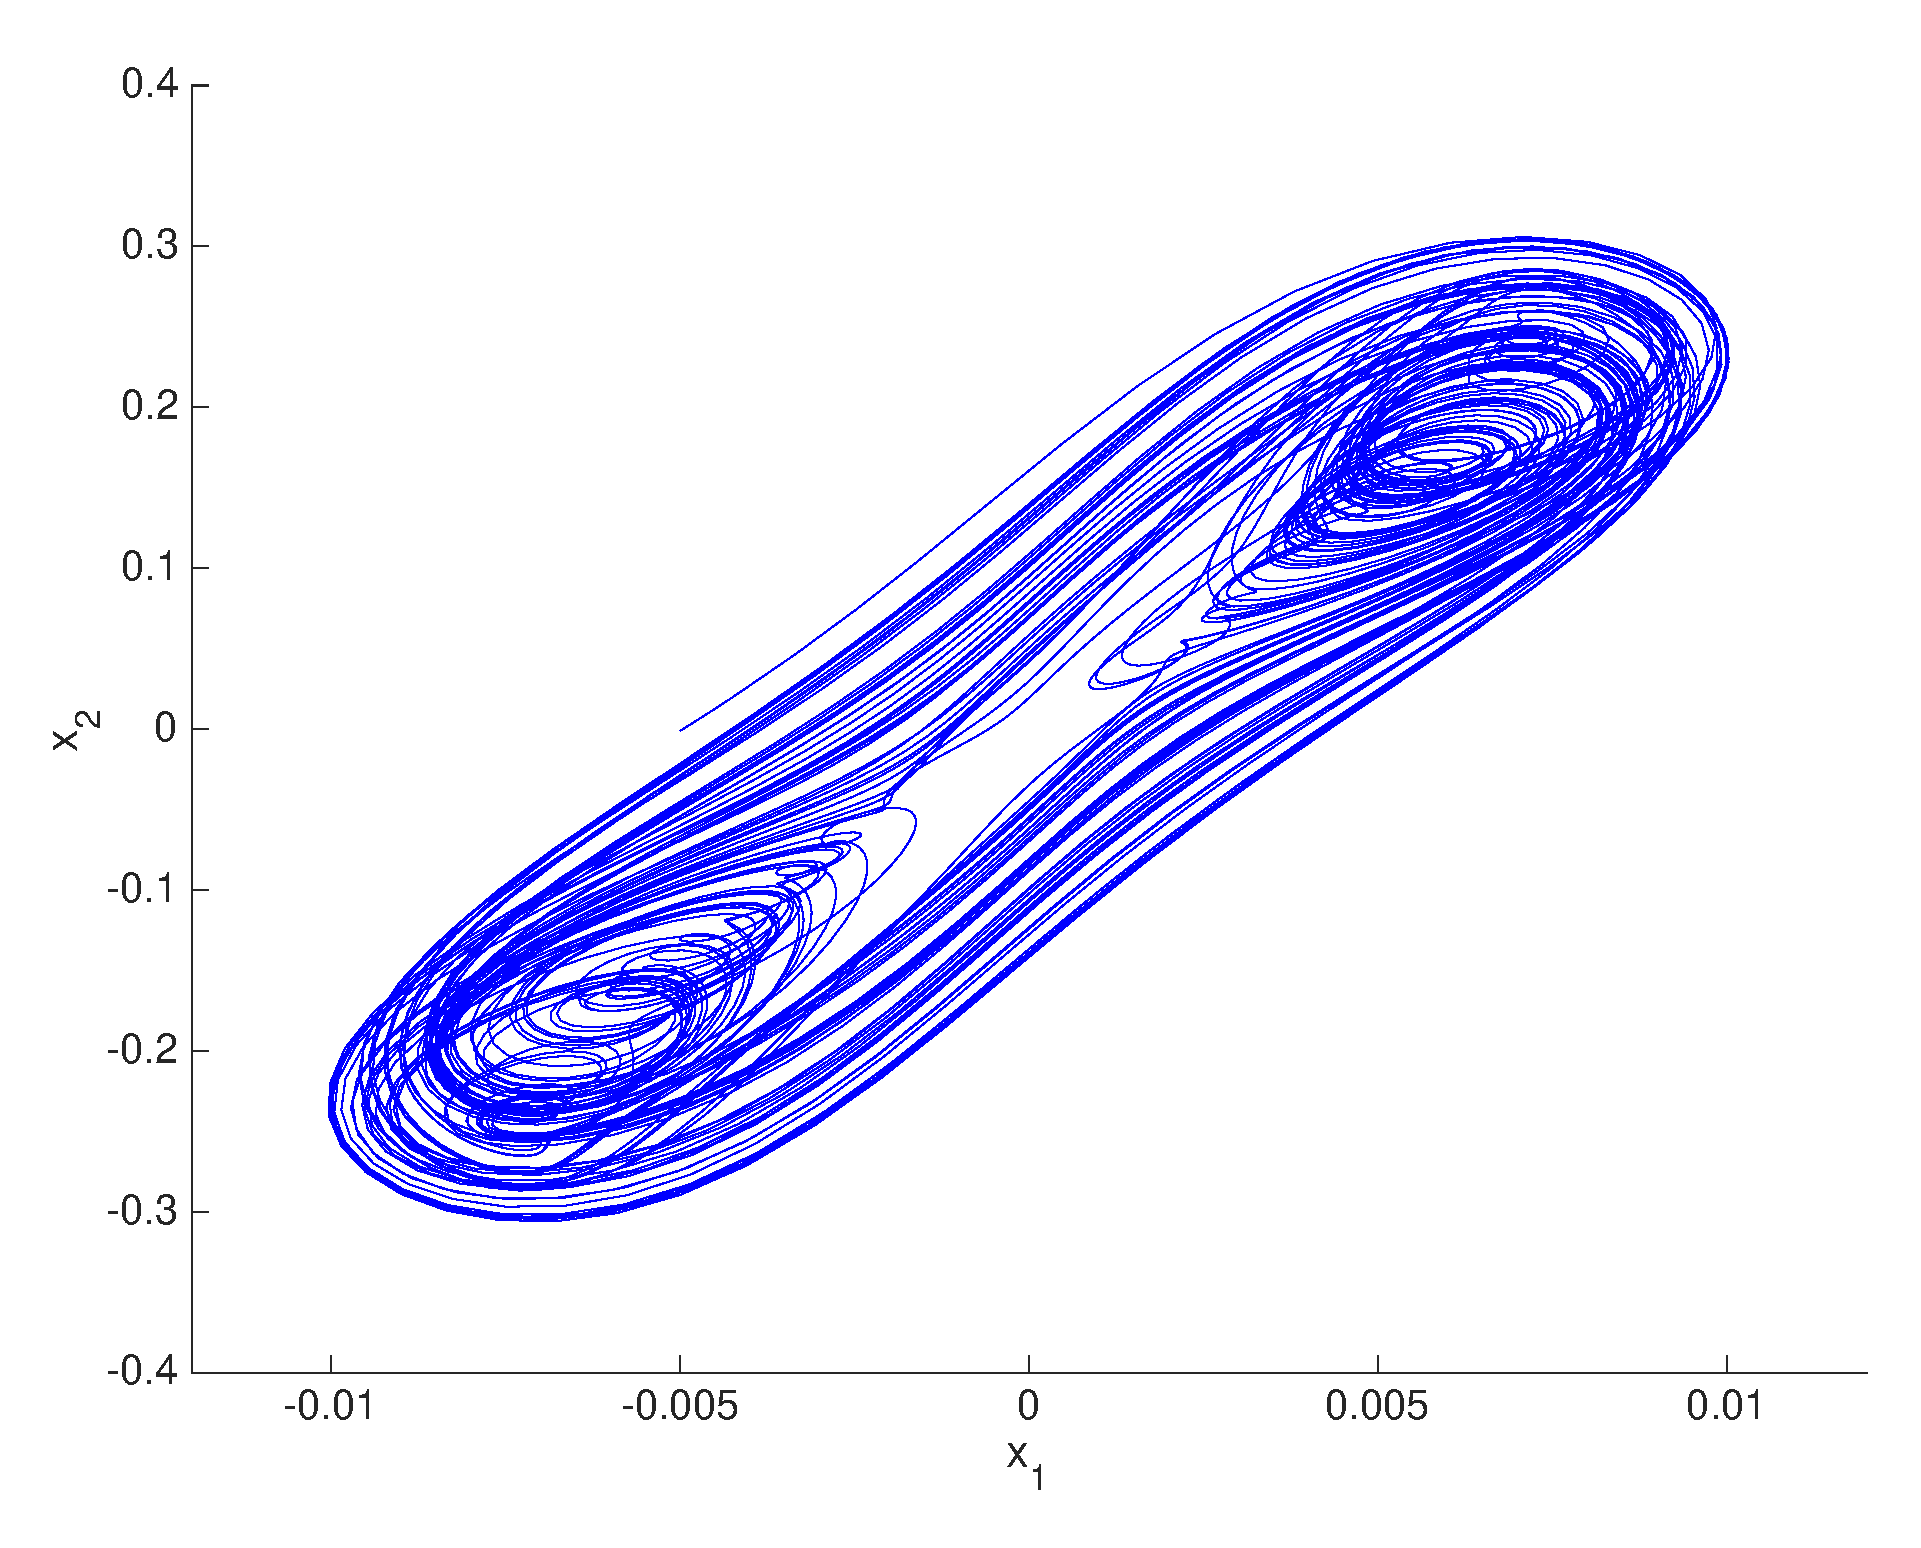
\includegraphics[width=\textwidth]{matcont/StranoAttrattore2D}
        \caption{L'orbita vista ``dall'alto'', sul piano $x_1 x_2$.}
    \end{subfigure}
    \caption{Lo strano attrattore che si ottiene simulando il sistema per $\bar{R}=29.5 \Omega, \omega = 3.1415$.}
    \label{fig:strano-attrattore}
\end{figure}
